% Figures for SO(3) Tube Smoothing Paper
% All figures generated with font size 15, Times New Roman, light color style

\begin{figure}[htbp]
\centering
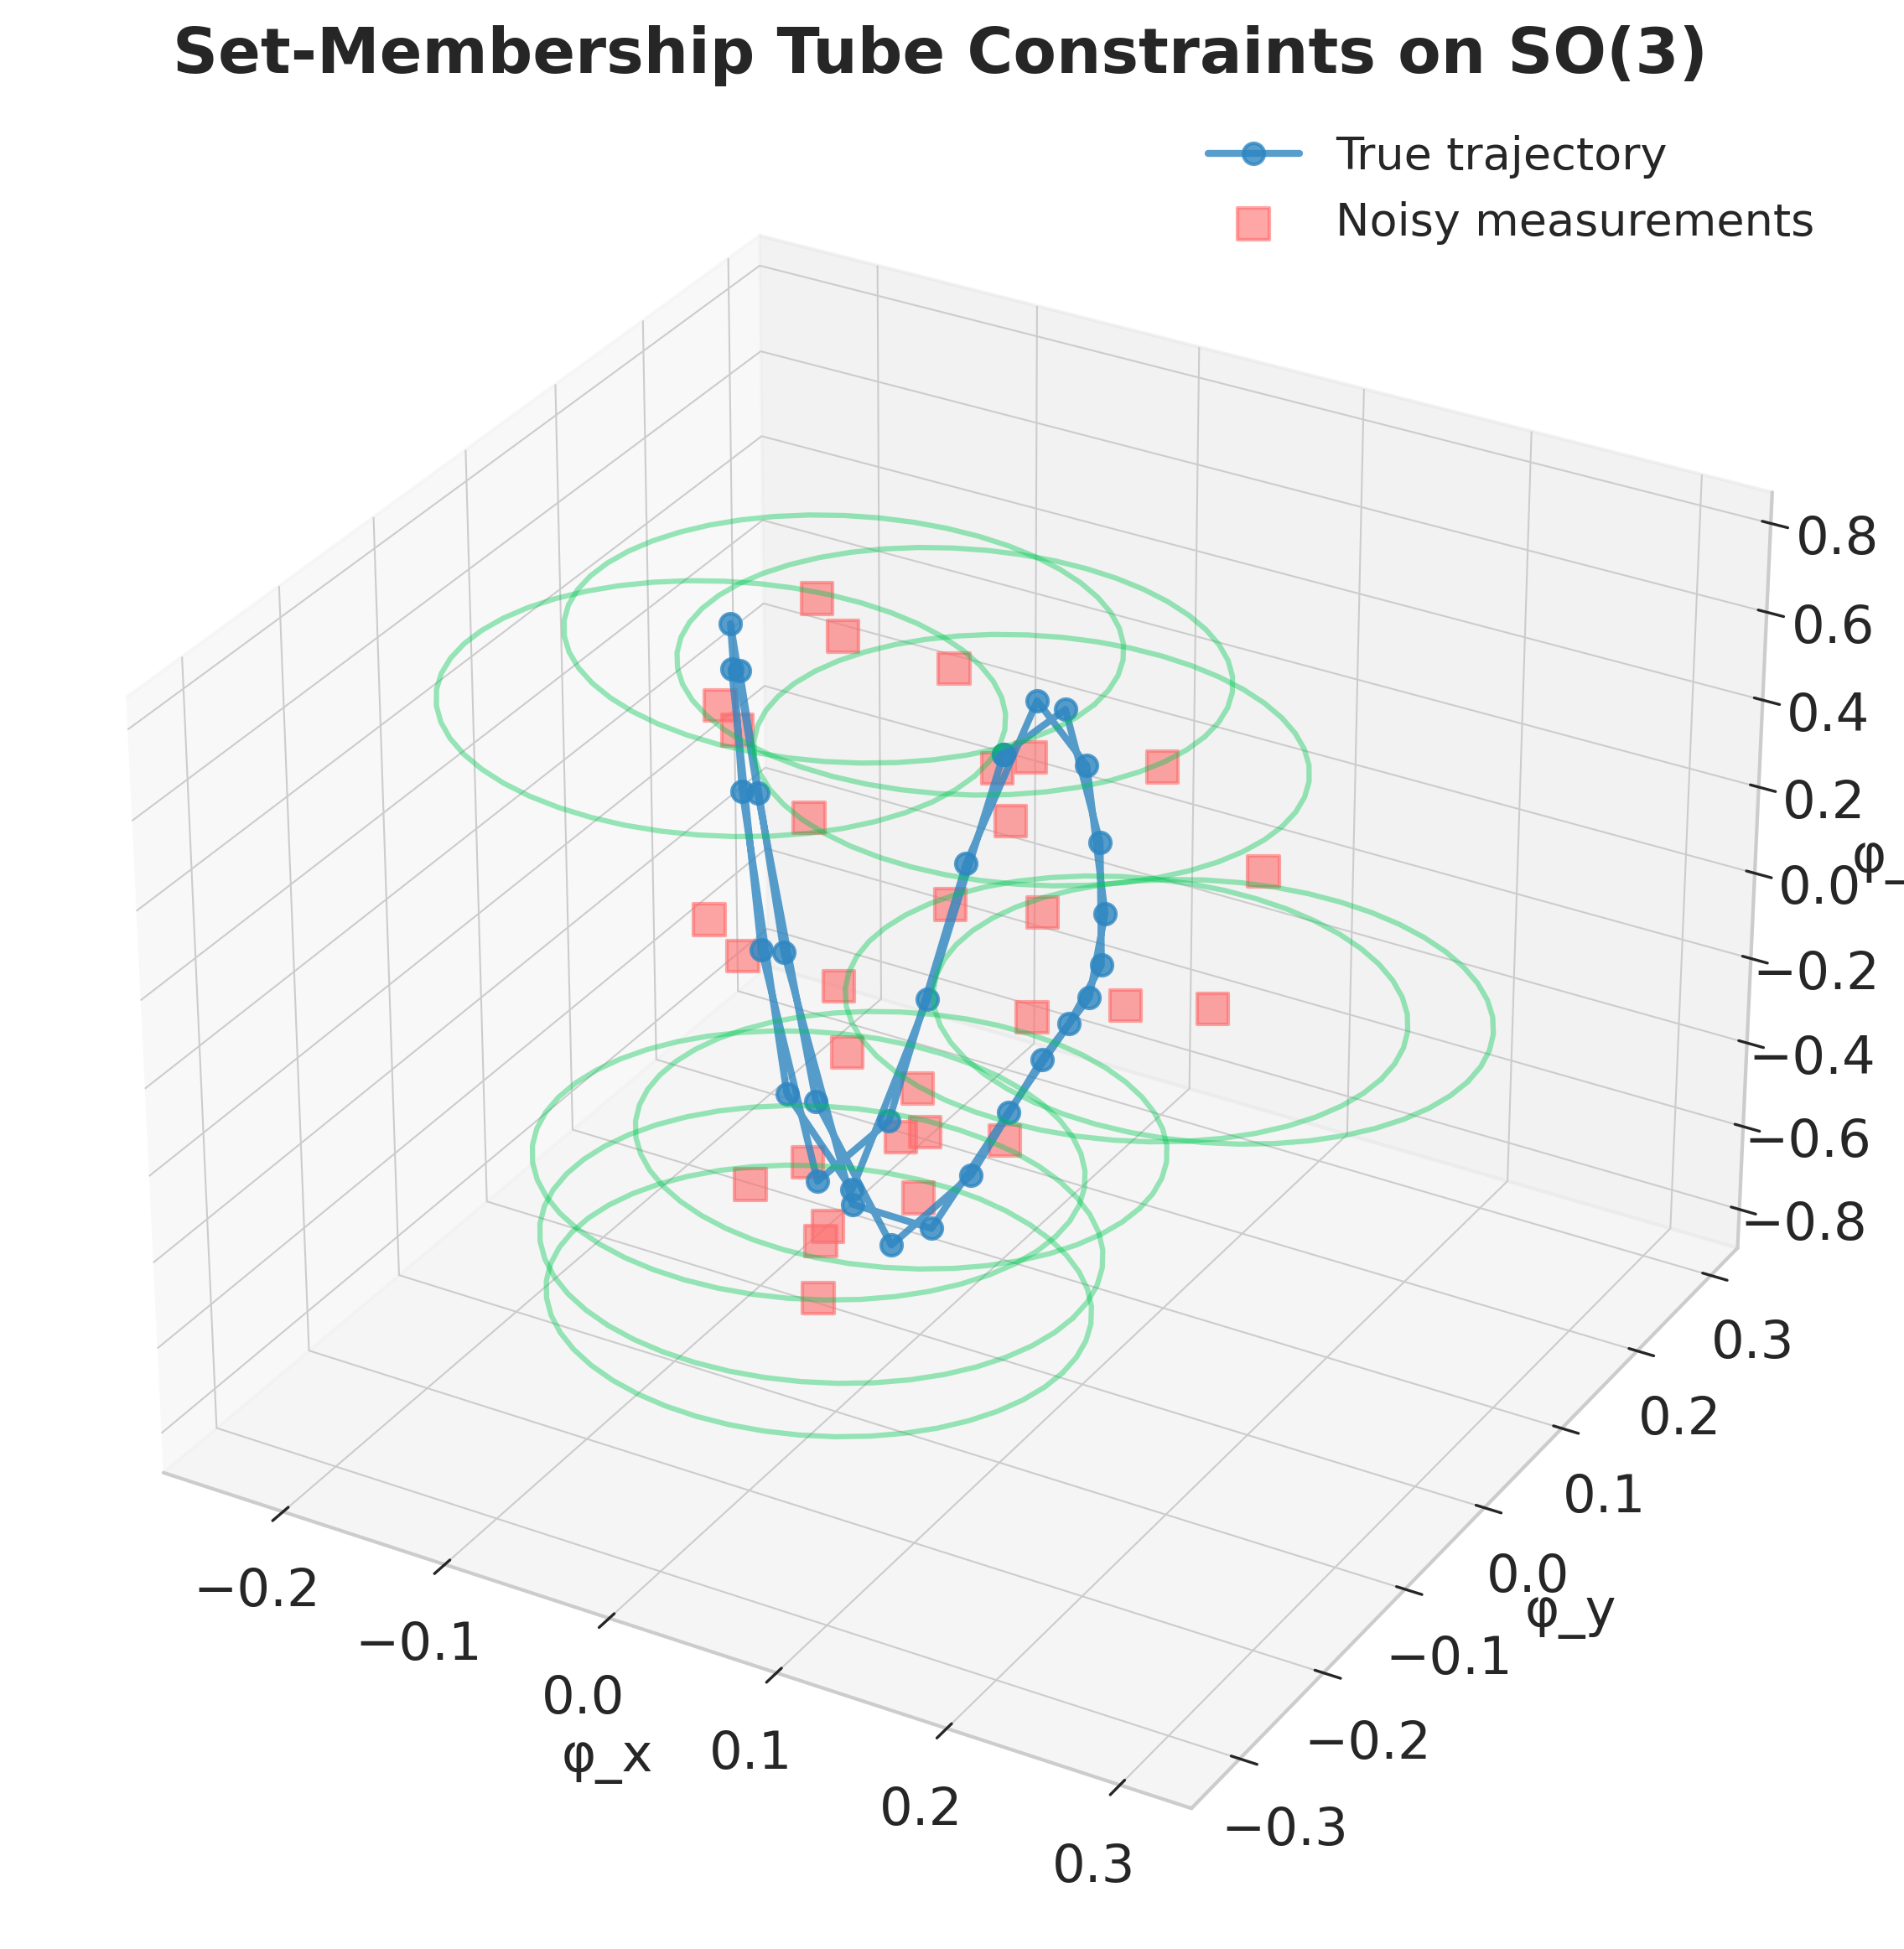
\includegraphics[width=0.9\textwidth]{figures/fig1_tube_constraints.png}
\caption{Set-membership tube constraints on SO(3). Each measured rotation must lie within a geodesic ball (tube) of radius $\epsilon_i$ around the smoothed rotation. The green circles represent tube boundaries around noisy measurements (red stars), while the blue line shows the true underlying trajectory.}
\label{fig:tube}
\end{figure}

\begin{figure}[htbp]
\centering
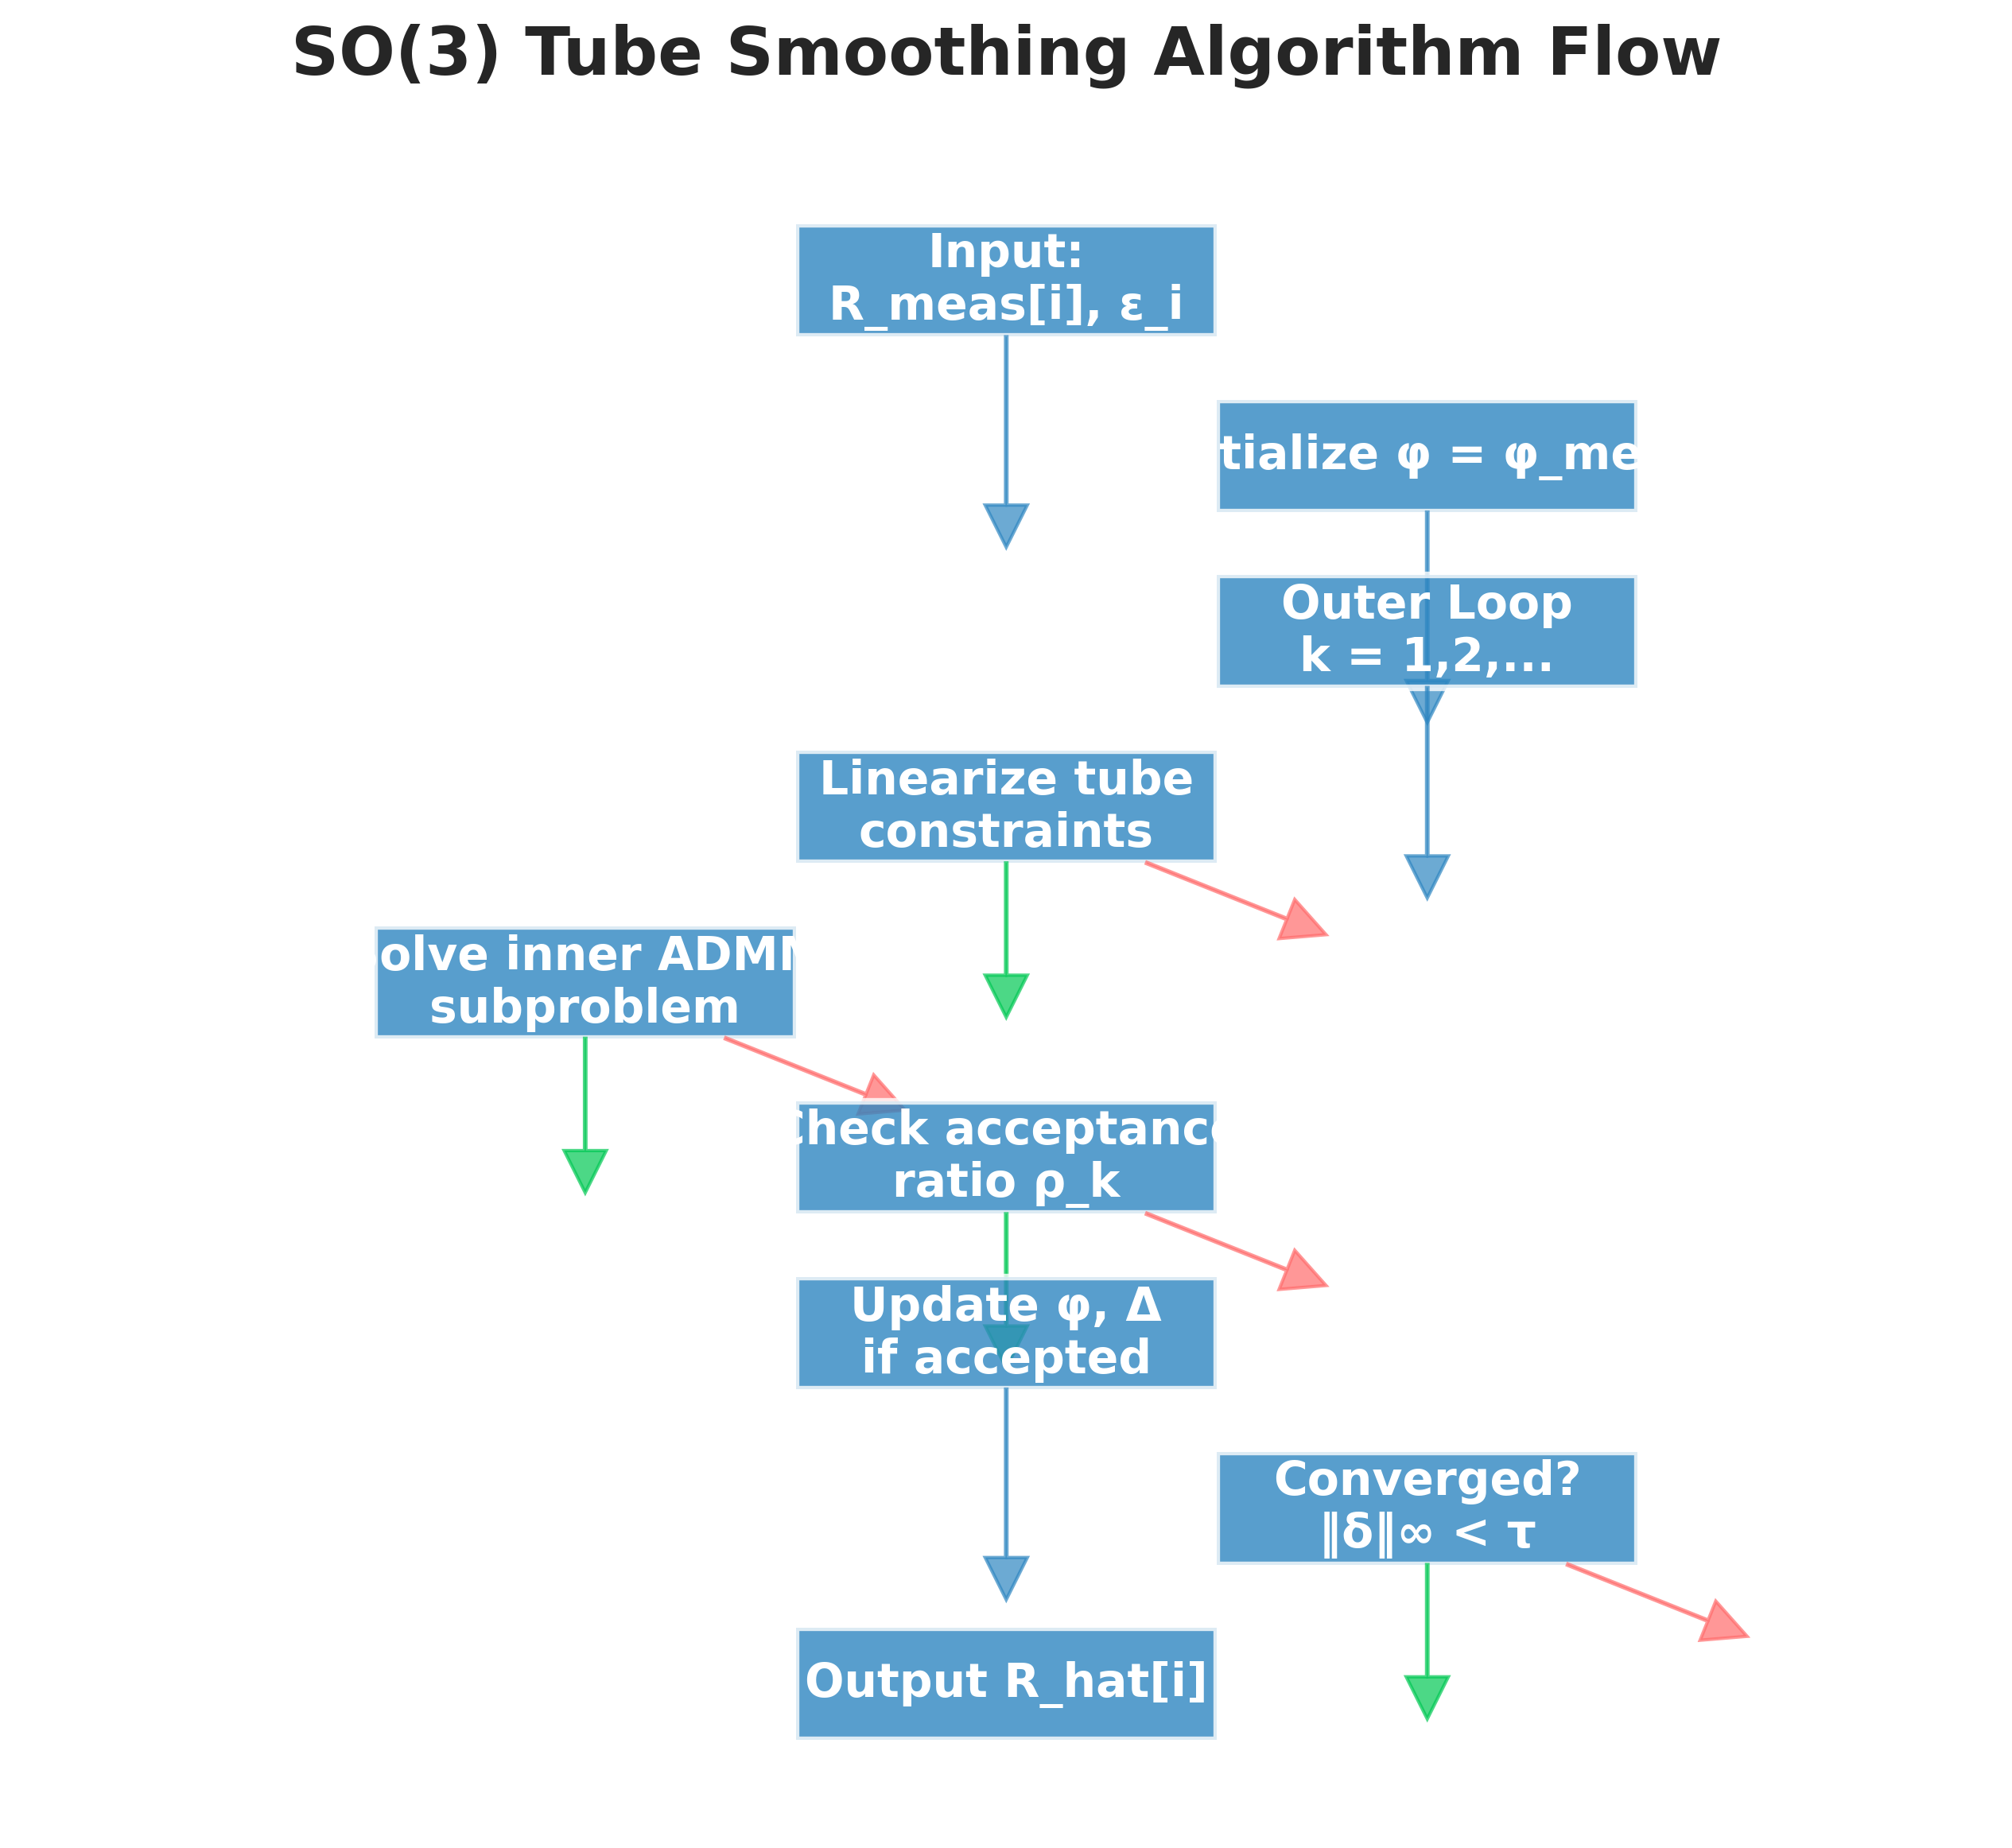
\includegraphics[width=0.95\textwidth]{figures/fig2_algorithm_flow.png}
\caption{Algorithm flow for SO(3) tube smoothing. The outer loop performs sequential convexification with trust-region management, while the inner ADMM solver efficiently handles the SOCP subproblem. Decision points are shown with branching arrows (green for accept, red for reject).}
\label{fig:algorithm}
\end{figure}

\begin{figure}[htbp]
\centering
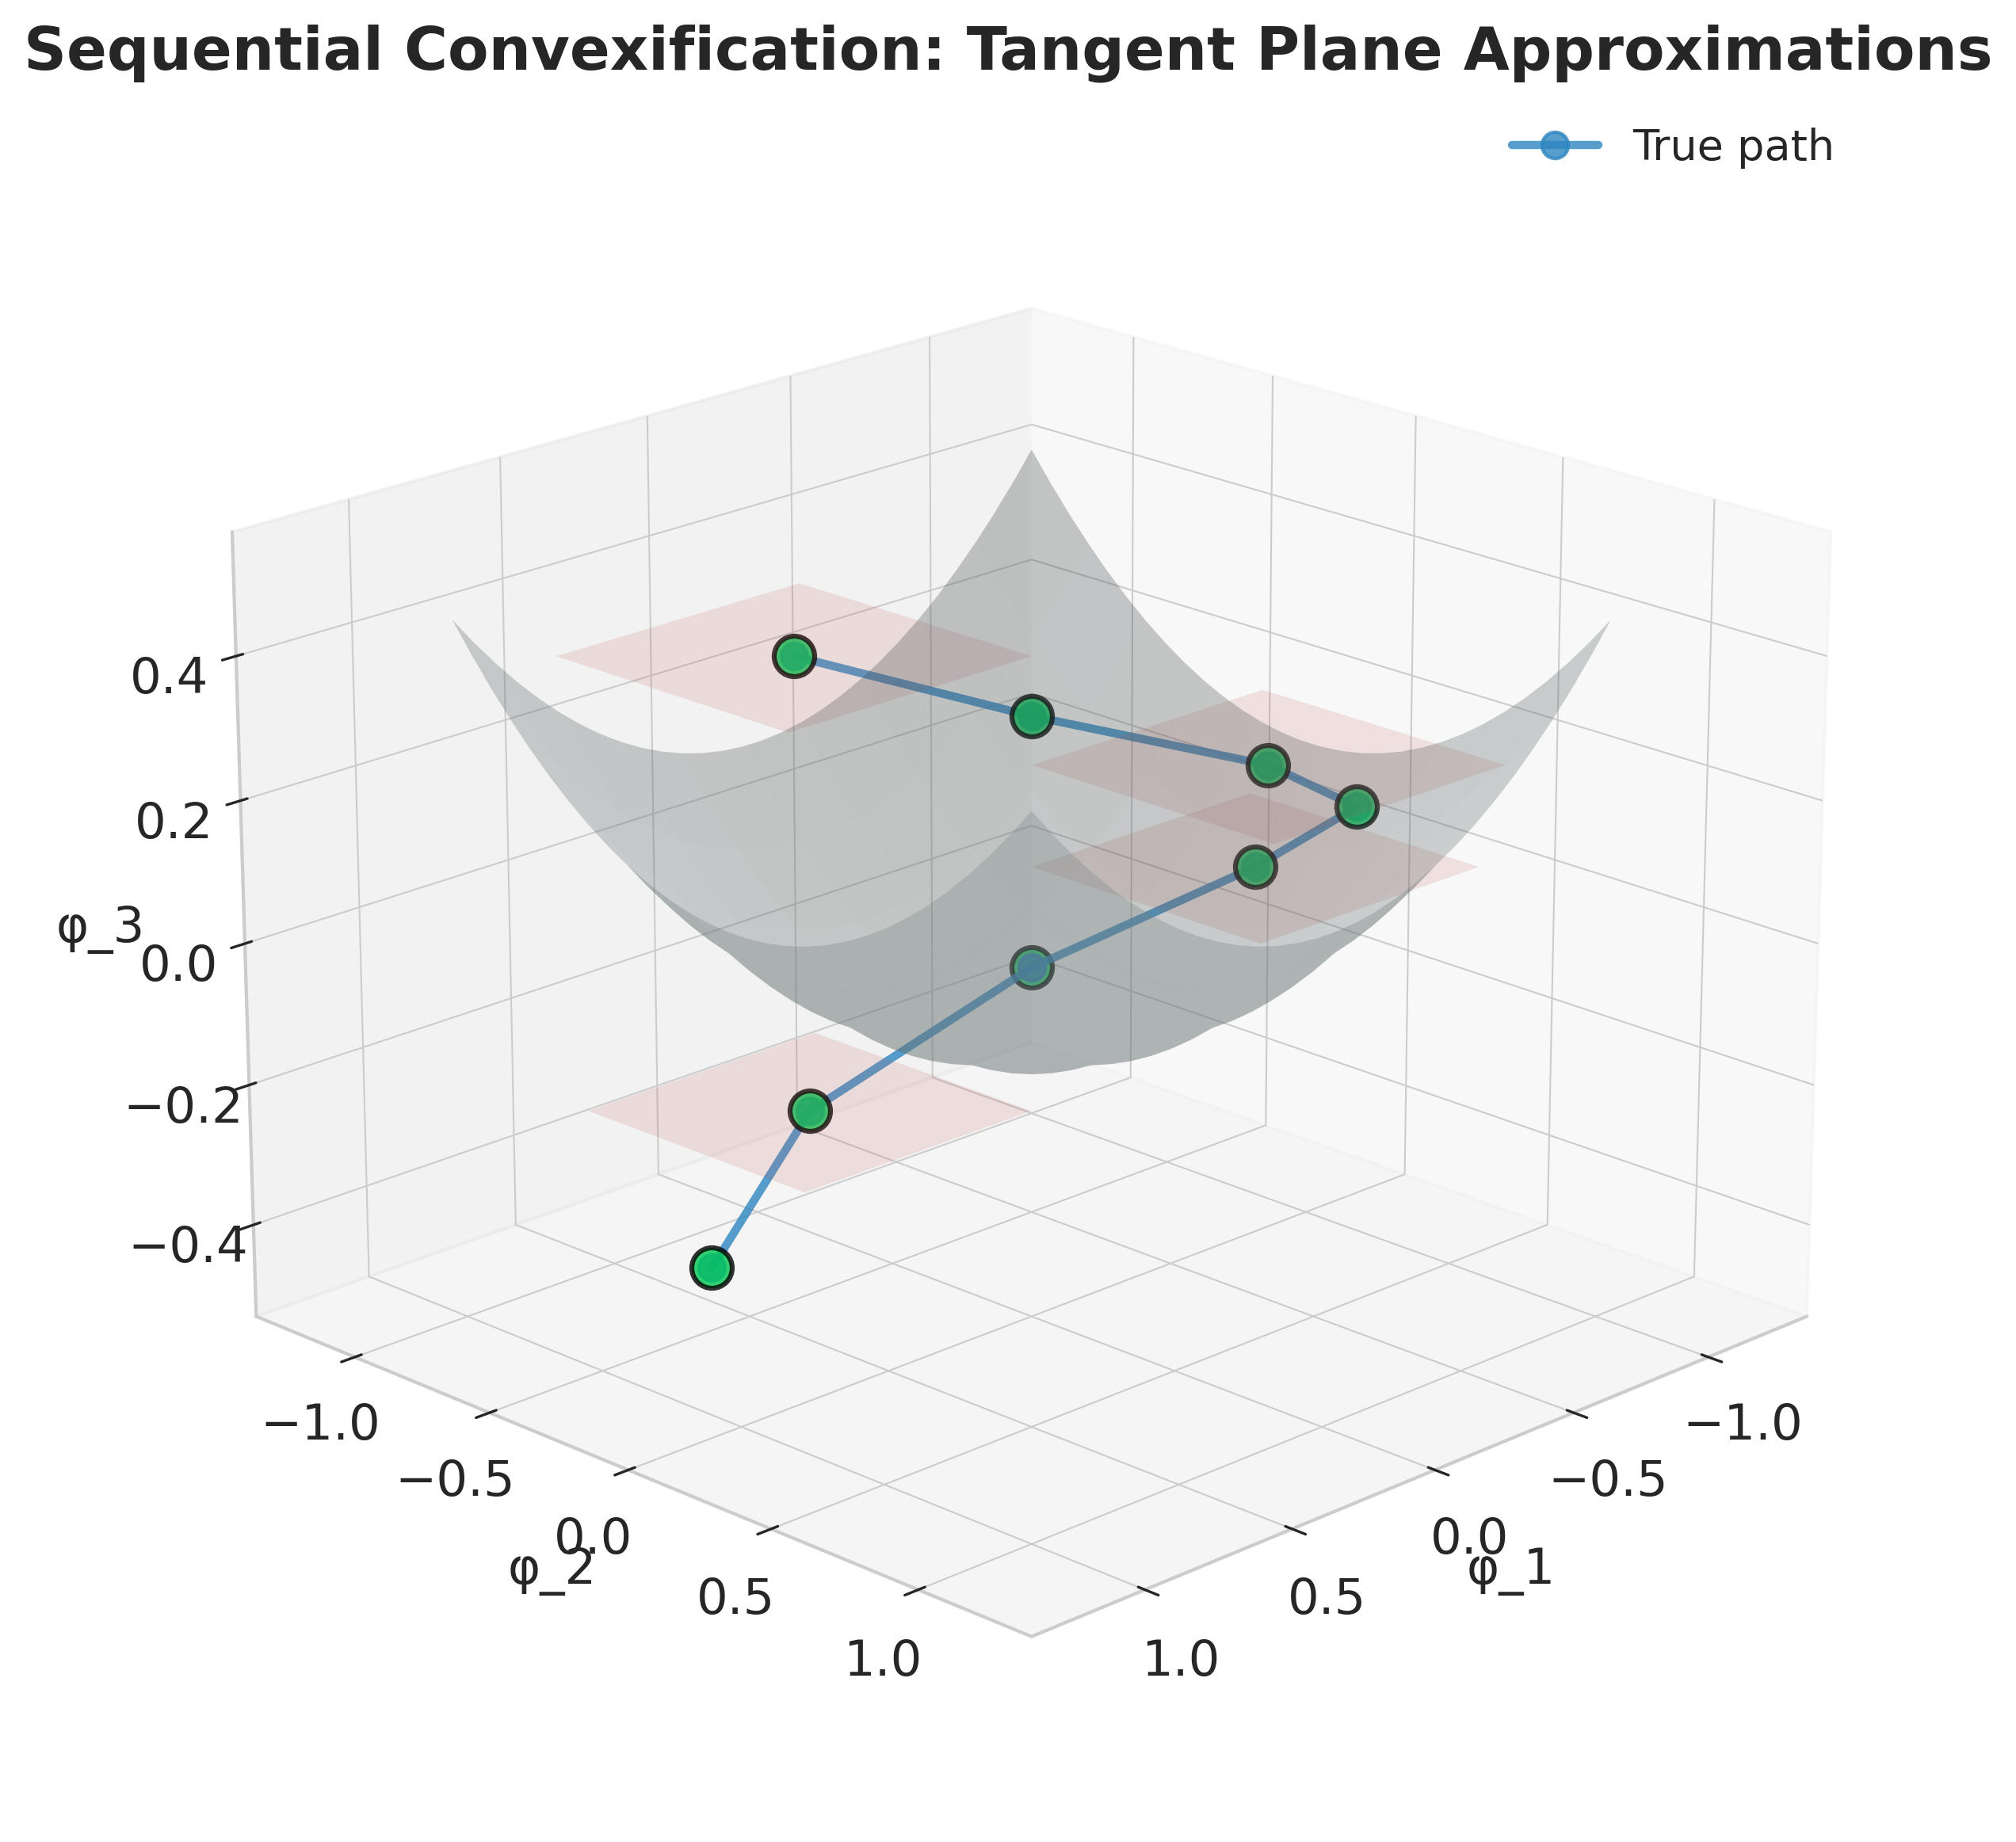
\includegraphics[width=0.85\textwidth]{figures/fig3_convexification.png}
\caption{Sequential convexification on SO(3). The gray curved surface represents the non-convex tube constraint boundary. At each iteration, we approximate the constraint using a tangent plane (red surfaces) at the current iterate (green circles), forming a convex SOCP subproblem that can be solved efficiently.}
\label{fig:convexification}
\end{figure}

\begin{figure}[htbp]
\centering
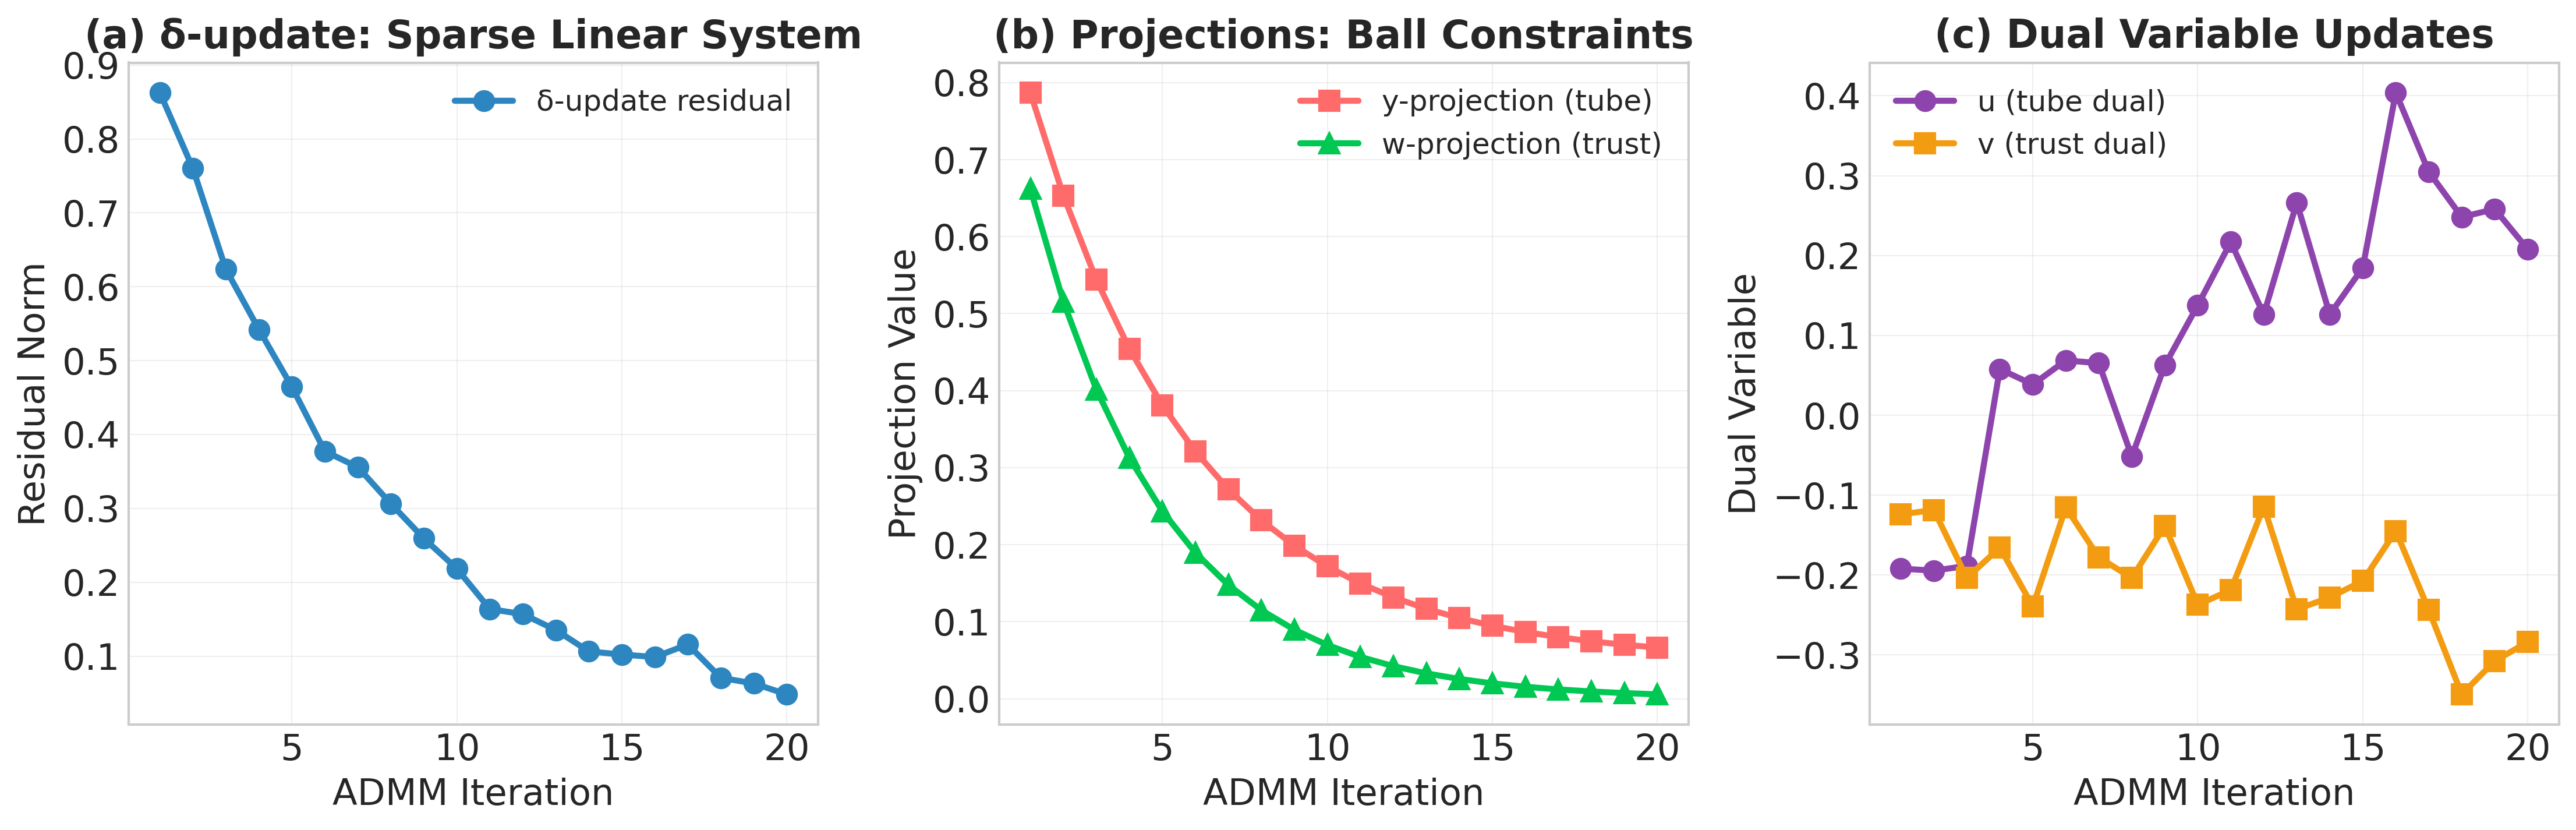
\includegraphics[width=0.95\textwidth]{figures/fig4_admm_updates.png}
\caption{ADMM update mechanism. (a) $\delta$-update solves a sparse linear system using the block-banded Hessian structure. (b) Projection updates enforce tube and trust-region constraints via inexpensive ball projections. (c) Dual variables ($\mathbf{u}$ for tubes, $\mathbf{v}$ for trust regions) ensure constraint satisfaction.}
\label{fig:admm}
\end{figure}

\begin{figure}[htbp]
\centering
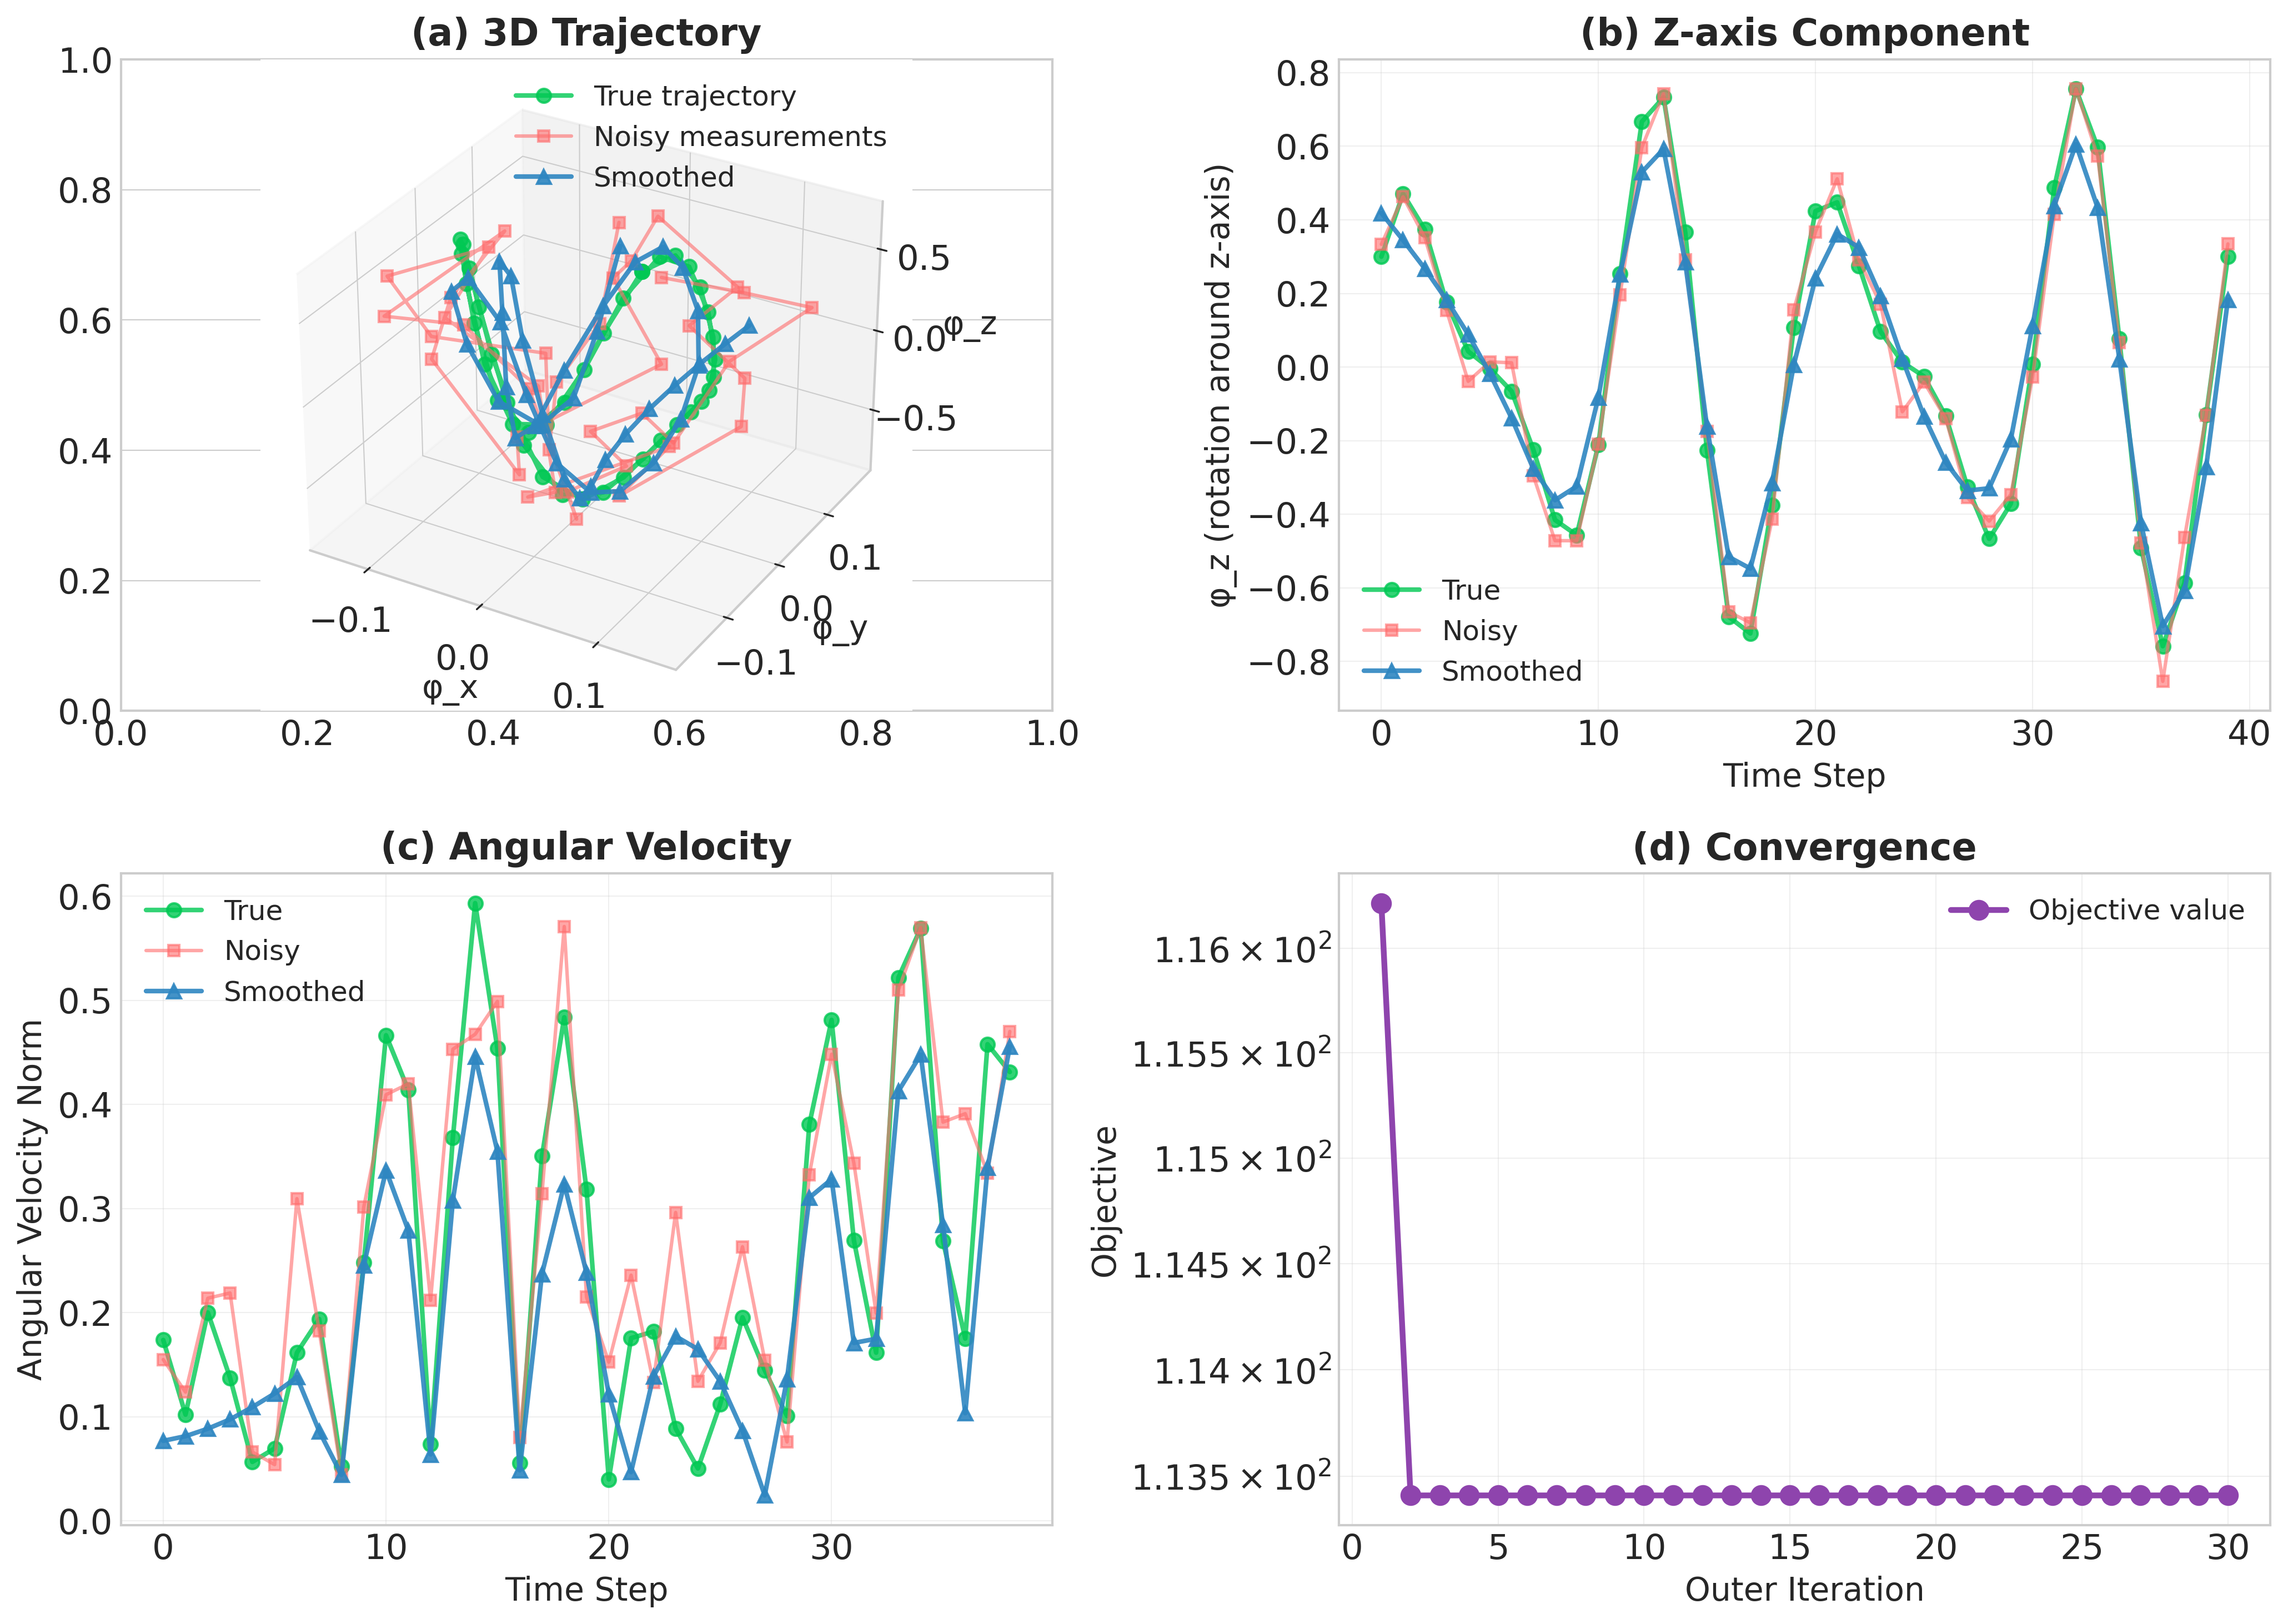
\includegraphics[width=0.95\textwidth]{figures/fig5_smoothing_example.png}
\caption{Complete smoothing example on synthetic data. (a) 3D trajectory showing true path (green circles), noisy measurements (red stars), and smoothed result (blue triangles). (b) Individual component (z-axis rotation) showing noise reduction. (c) Angular velocity demonstrating smoothness improvement. (d) Convergence plot showing objective value decrease over 30 outer iterations.}
\label{fig:example}
\end{figure}
